\documentclass{beamer}
\usepackage{animate}
\usepackage{amsmath}
\usepackage{tikz}
\usetheme{Madrid}
\usepackage{tikz}
\usepackage{soul}
\usepackage[normalem]{ulem}
\graphicspath{{./figures/}}

\useinnertheme{circles}
%Information to be included in the title page:
\title{Measuring Changes in \sout{Pol II Speed} RNA Metabolism Kinetic Rates from Total RNA-seq}
\author{Jakub Koubele}
\institute{Progress Report}
\date{3rd February, 2026}

\renewcommand{\insertshortauthor}{Jakub Koubele}  
\renewcommand{\insertshorttitle}{RNA metabolism kinectics}
\renewcommand{\insertshortdate}{3rd February, 2026} % Define custom text for 3rd block

\usepackage{amsthm}
\newcommand*{\QED}{\hfill\ensuremath{\blacksquare}}





\begin{document}
	\frame{\titlepage}
	
	
	\begin{frame}
		\frametitle{Introduction}	
		\pause
		
		
		\begin{itemize}
			
			
			\item I wanted to estimate changes in transcription elongation speed, but the project got a bit more complex.
			\vspace{2em}
			\begin{center}
				\includegraphics[width=4cm]{pol}
			\end{center}
			
			
		\end{itemize}		
		
	\end{frame}
	
	\begin{frame}
		\frametitle{Total RNA}	
		\pause
		
		\begin{itemize}
			\item Total RNA is a combination of nascent and mature RNA.
			
			
			
			\begin{center}
				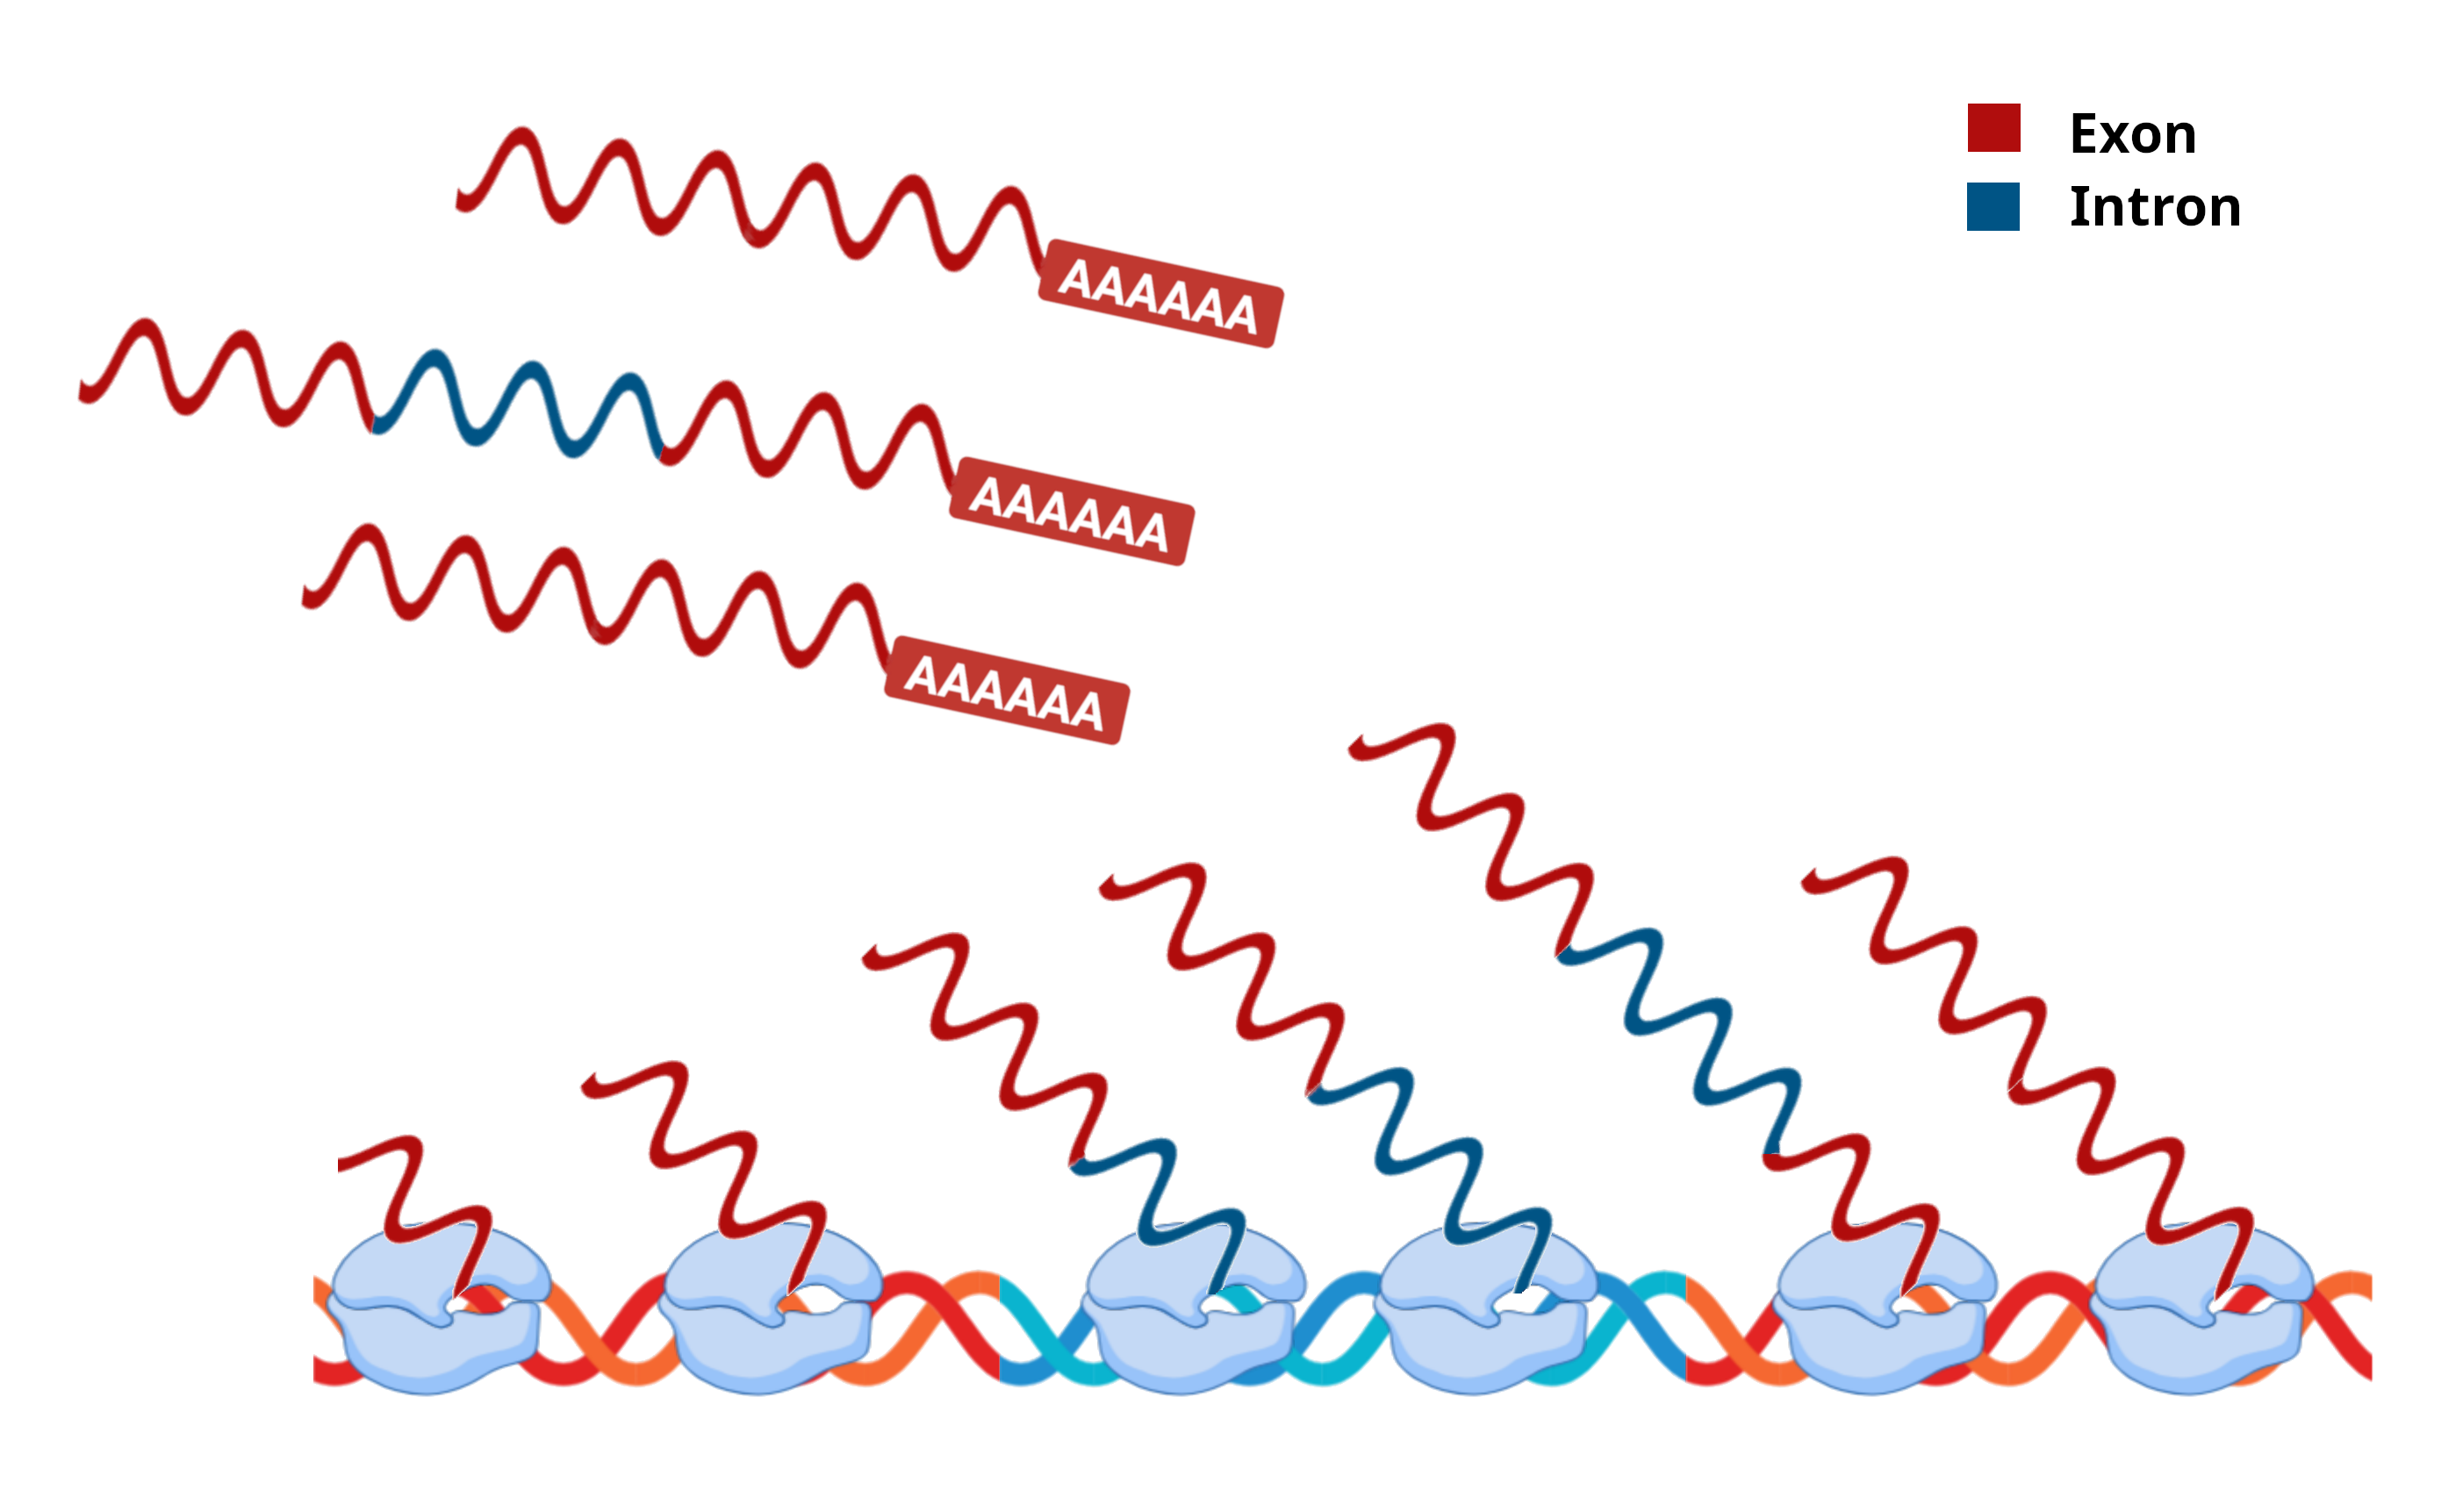
\includegraphics[width=9cm]{total_rna}
			\end{center}
			
			\pause
			
			\item In shorts read RNA-seq, unfinished transcripts and introns exhibit 5' coverage bias (compared to uniform coverage from finished ones).
			
		\end{itemize}
		
	\end{frame}
	
	
	\begin{frame}
		\frametitle{RNA kinetics}	
		\pause
		
		Several kinetic rates influence the total RNA composition:
		\pause
		\begin{enumerate}
			\item Expression rate (how often is the gene transcribed).
			\pause
			\item Transcription elongation speed.
			\pause
			\item Speed of intron splicing.
			\pause
			\item Degradation rate of mature RNA.
			\pause
		\end{enumerate}
		
	\end{frame}
	
	\begin{frame}
		\frametitle{Changes in expression rate}	
		\pause
		\begin{itemize}
			\item Changes in gene expression (i.e., transcription initiation rate) scale the abundance of both nascent and mature RNA of that gene.	
		\end{itemize}	
		\begin{center}
			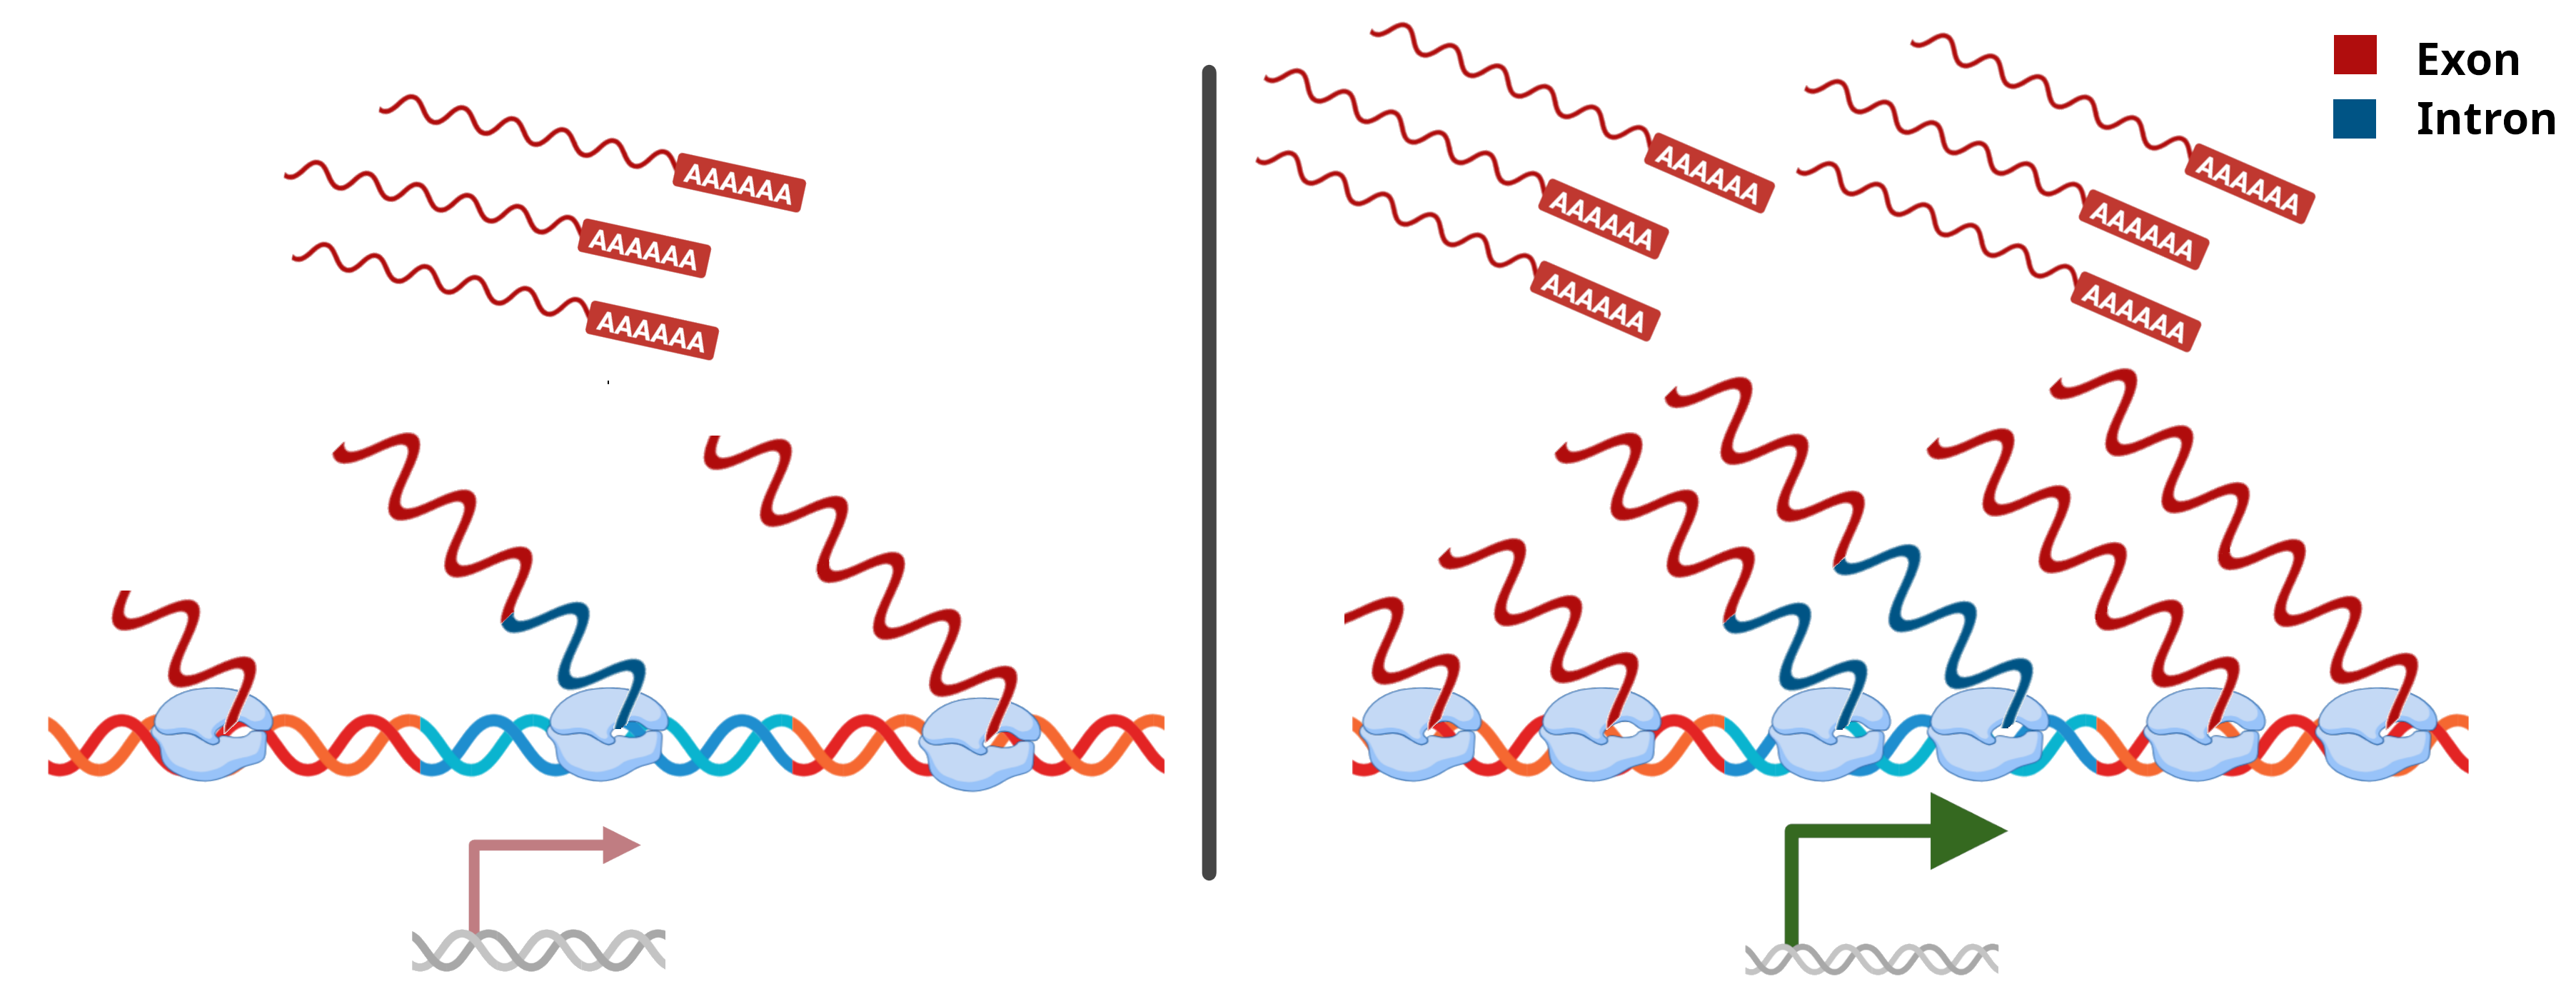
\includegraphics[width=11cm]{gene_expression}
		\end{center}
		
	\end{frame}
	
	\begin{frame}
		\frametitle{Changes in elongation speed}	
		\pause
		\begin{itemize}
			\item With a faster elongation (right), there are fewer polymerases currently transcribing the gene, compared to a slower elongation (left).
		\end{itemize}	
		\begin{center}
			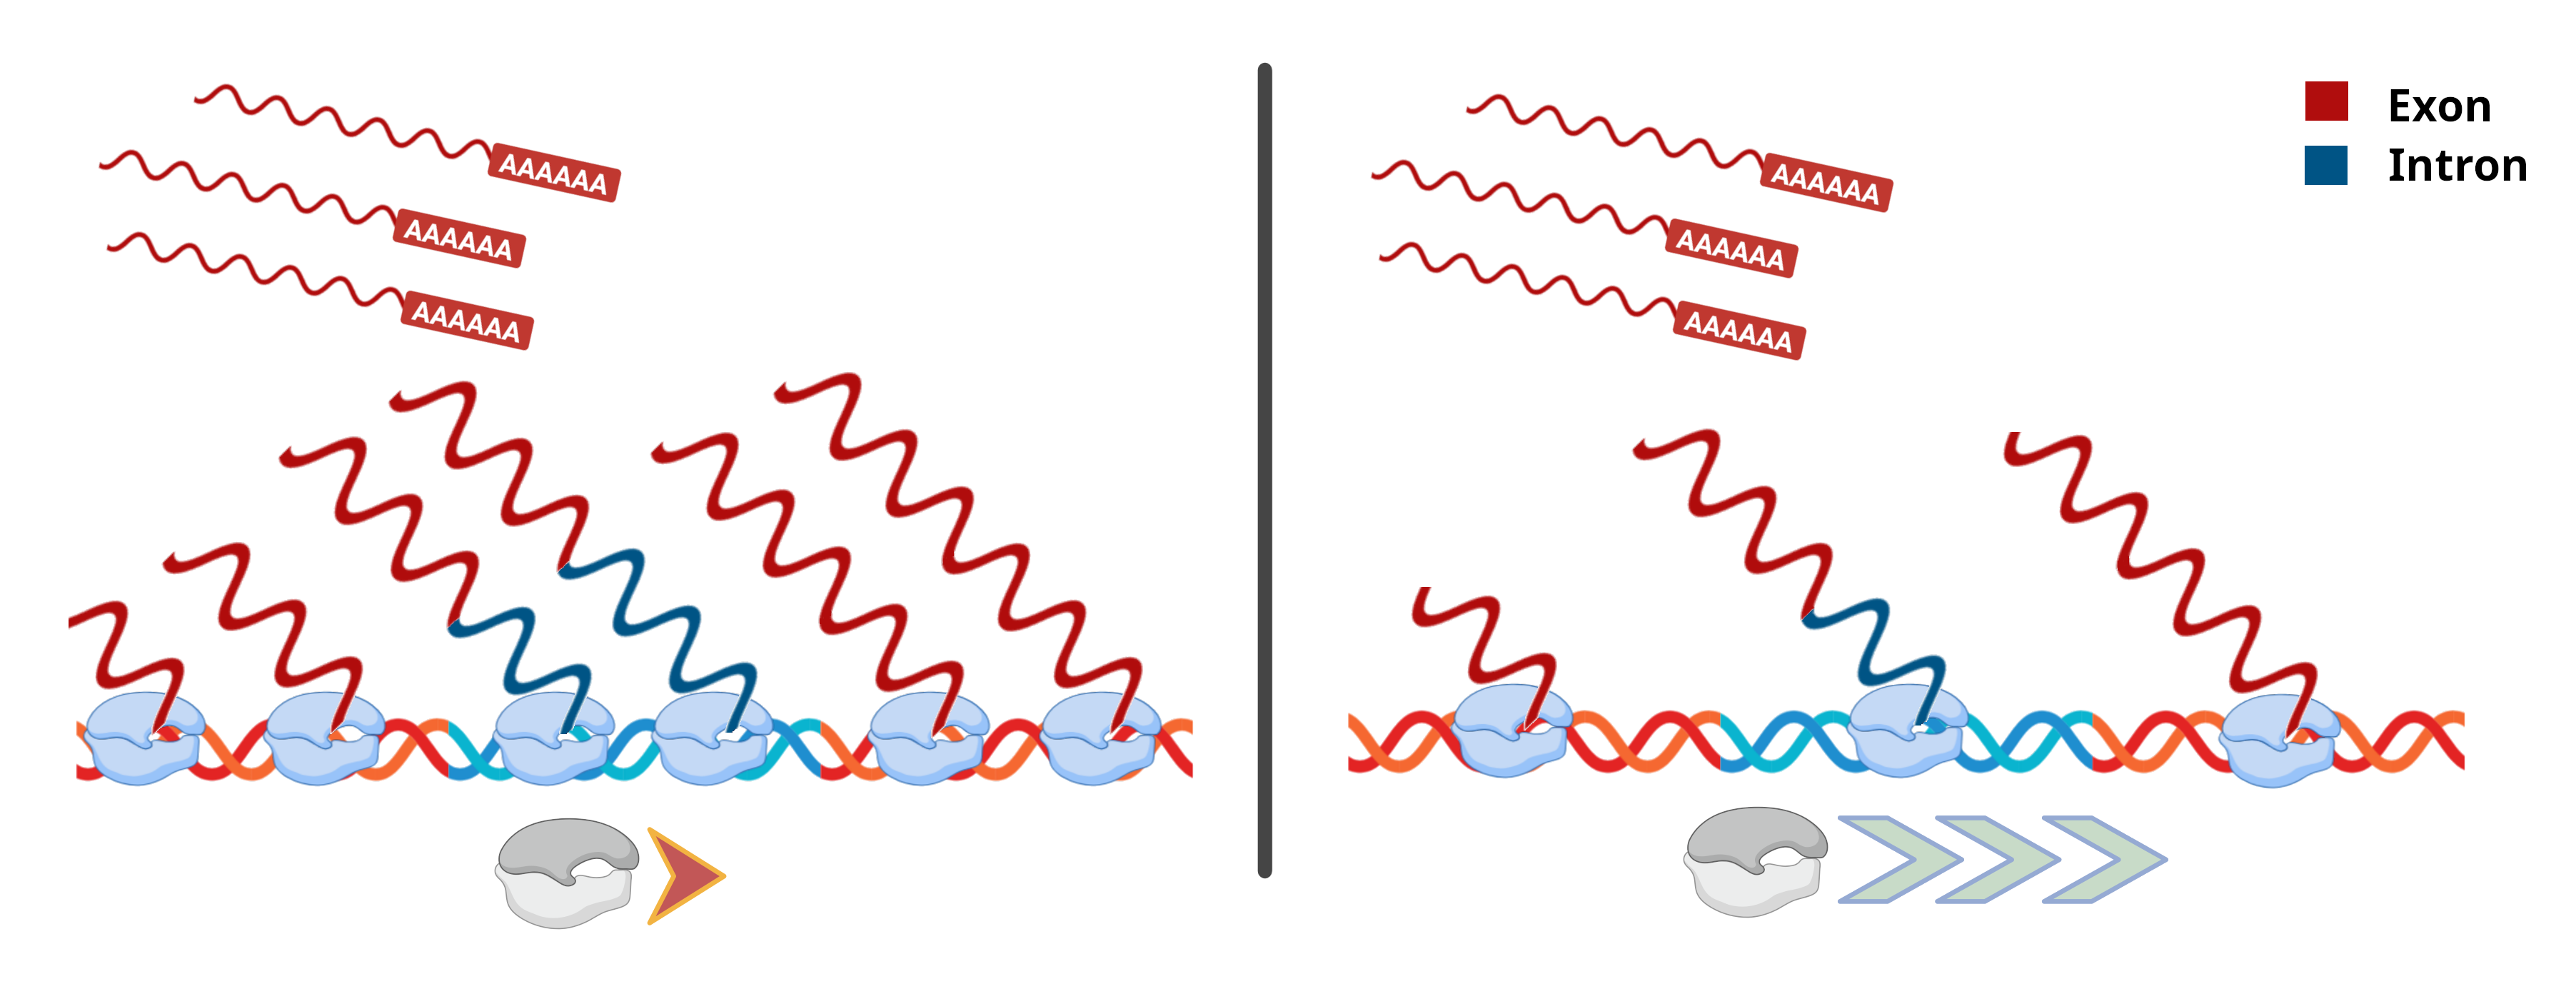
\includegraphics[width=11cm]{elongation_speed}
		\end{center}
		
	\end{frame}
	
	
	\begin{frame}
		\frametitle{Changes in intron splicing speed}	
		\pause
		\begin{itemize}
			\item With slower splicing (left), the sample will
			contains more unspliced introns.
		\end{itemize}	
		\vspace{1em}
		\begin{center}
			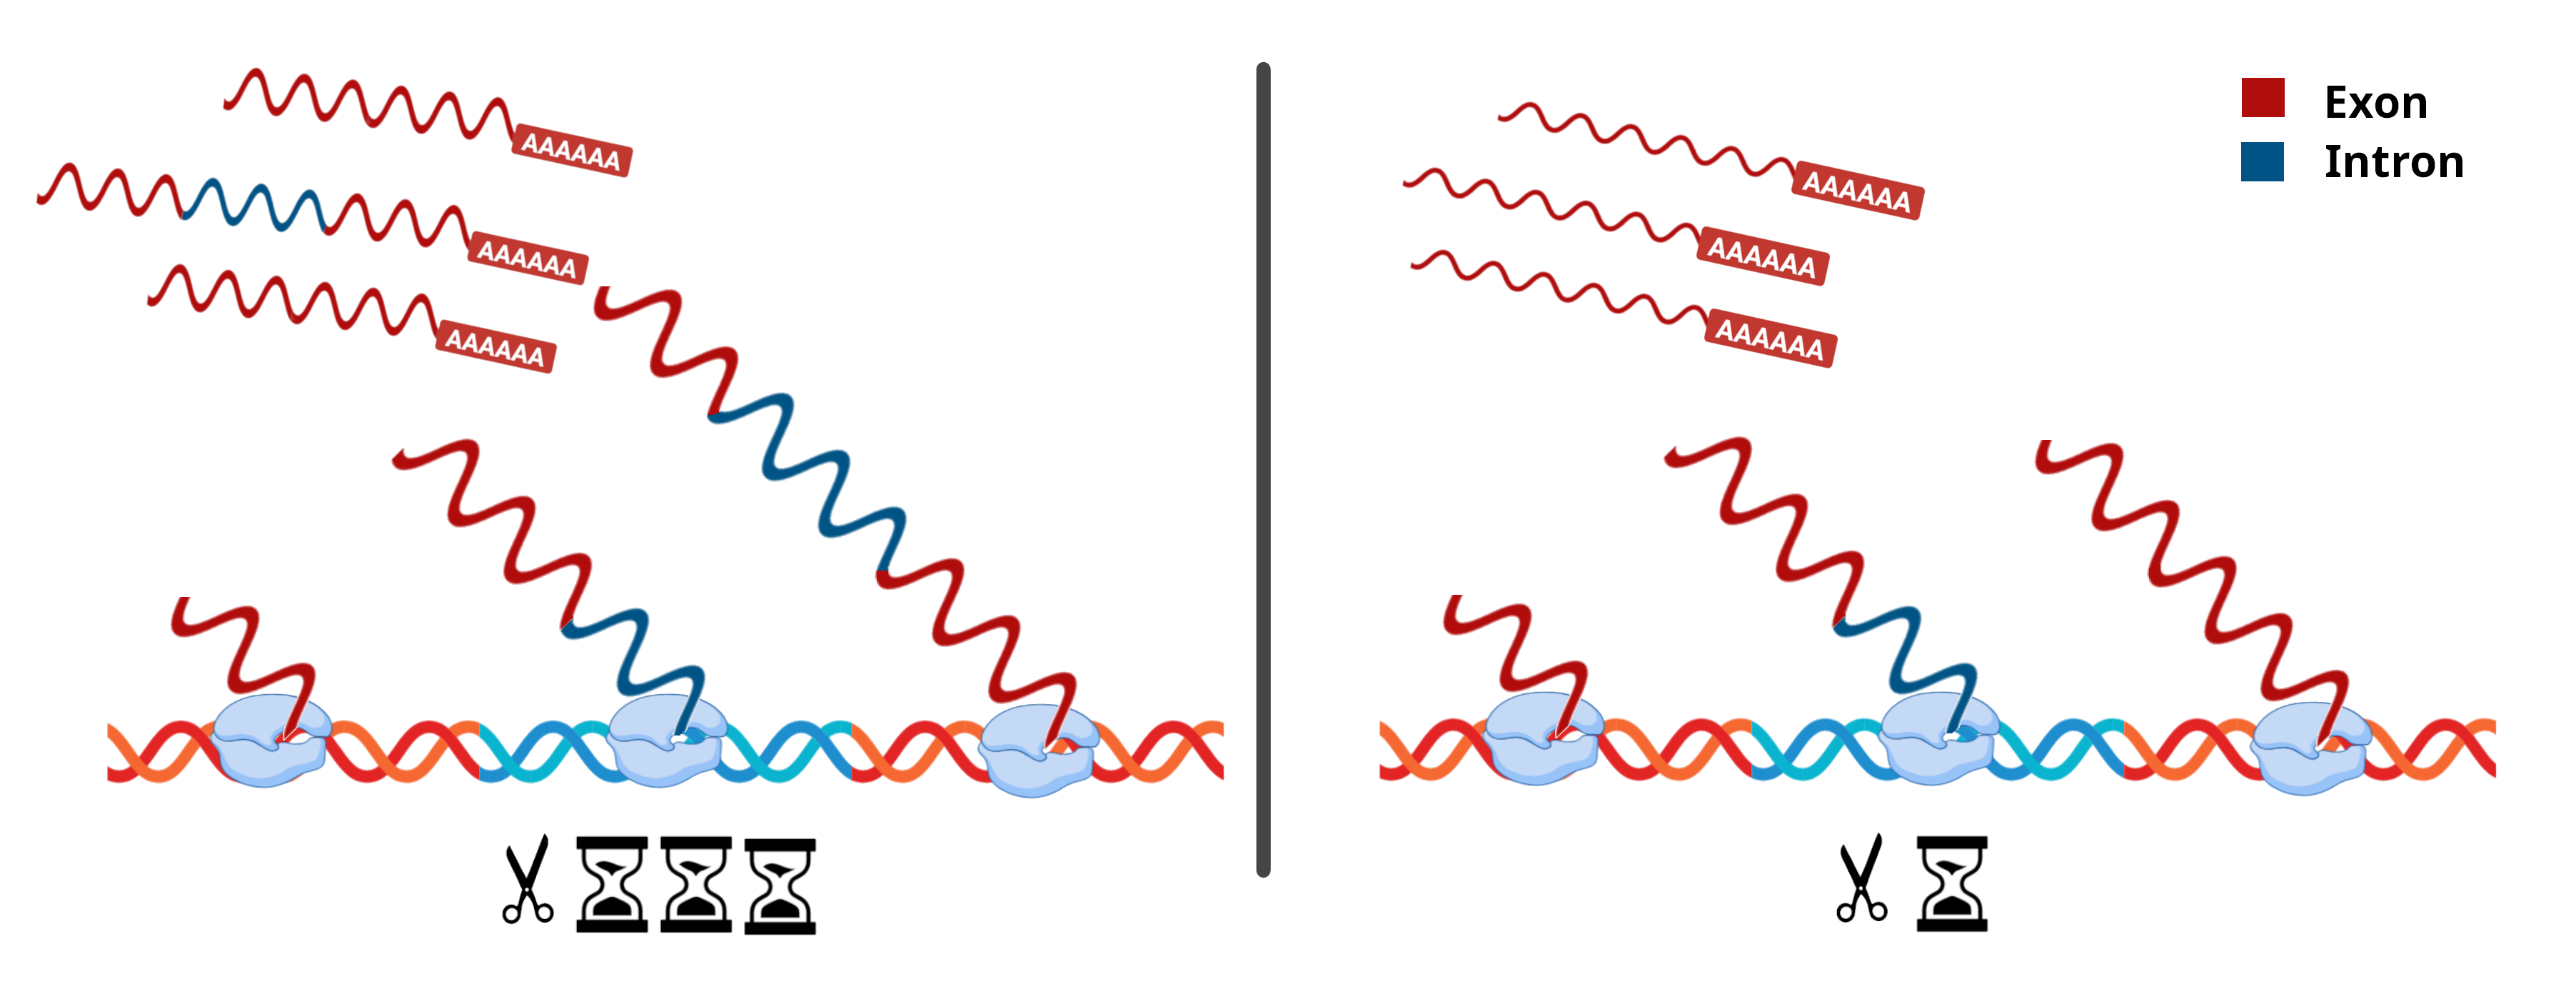
\includegraphics[width=11cm]{splicing_time}
		\end{center}
		
	\end{frame}
	
	
	\begin{frame}
		\frametitle{Changes in RNA degradation}	
		\pause
		\begin{itemize}
			\item With faster degradation (right), less mature RNA will be present in the sample.
		\end{itemize}	
		\vspace{1em}
		\begin{center}
			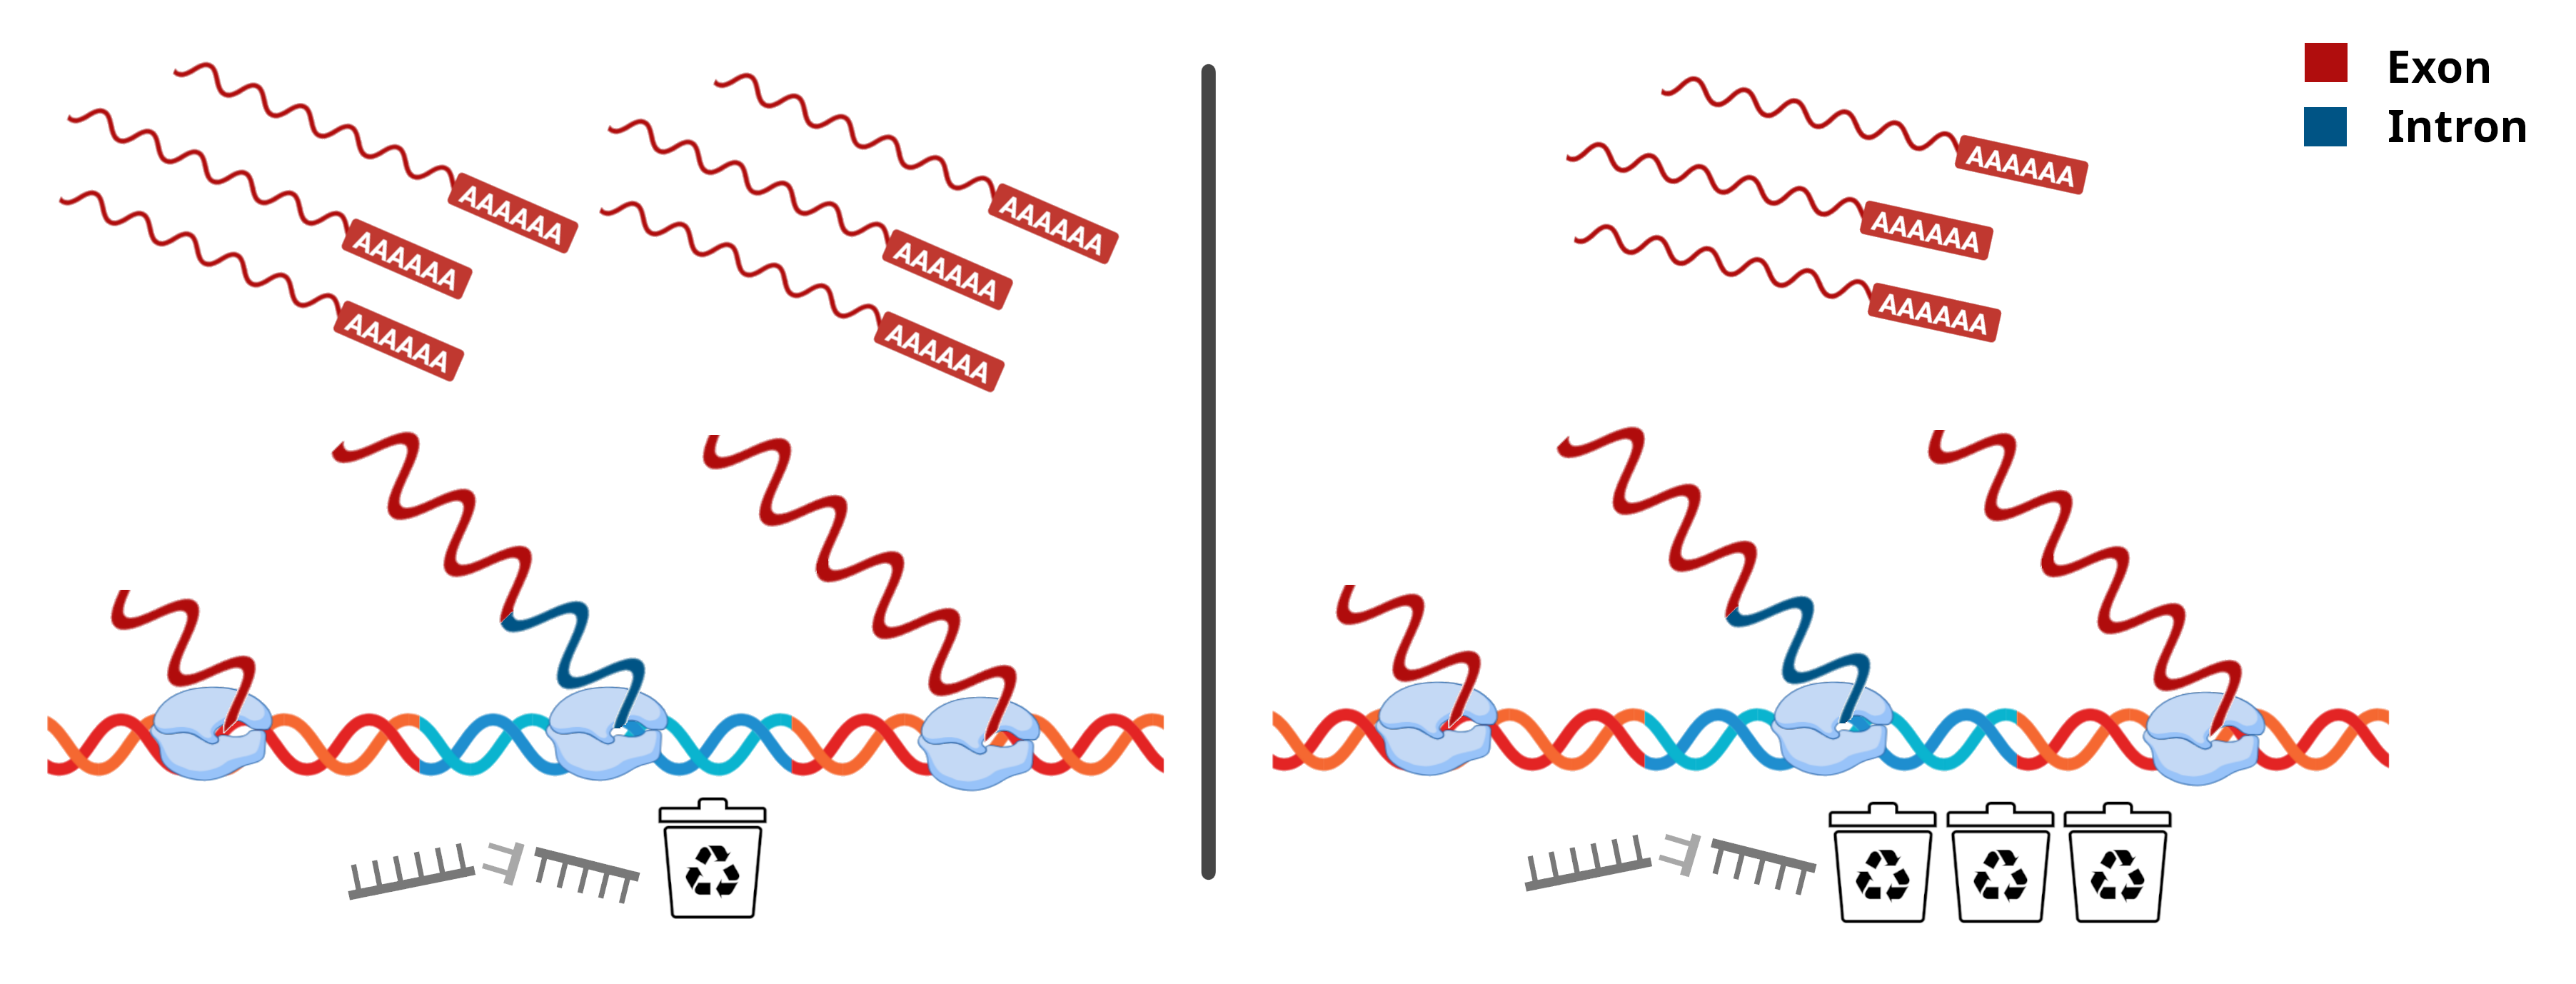
\includegraphics[width=11cm]{rna_degradation.png}
		\end{center}
		
	\end{frame}
	
	\begin{frame}
		\frametitle{RNA metabolism as a dynamic system}
		\pause
		We may model these four \textbf{quantities}:
		\begin{itemize}
			\item Nascent transcripts: $T_{nascent}$
			\item Mature transcripts: $T_{mature}$
			\item Nascent introns: $I_{nascent}$
			\item Unspliced (finished) introns: $I_{unspliced}$
		\end{itemize}	
		\pause
		Relevant \textbf{kinetic rates}:
		\pause
		\begin{itemize}
			\item Transcription initiation rate $\eta, [ \eta ] = \text{polymerases} \cdot s^{-1}$
			\pause
			\item Elongation speed $v, [ v ] = \text{bp} \cdot s^{-1}$
			\pause
			\item Intron splicing (and degradation) rate $k_{splice}, [k_{splice}] = s^{-1} $
			\pause
			\item RNA degradation rate $k_{deg}, [k_{deg}] = s^{-1}$
		\end{itemize}
		\pause
		\textbf{Other} symbols: 
		\begin{itemize}
			\item Gene and intron lengths: $L_{gene}$ and $L_{intron}$ (measured in $bp$).
		\end{itemize}
	\end{frame}
	
	\begin{frame}
		\frametitle{Metabolic reactions and steady state}
		\textbf{Metabolic reactions}:
		\pause
		\begin{itemize}
			\item $\text{production of } T_{nascent} = \text{production of } I_{nascent} = \eta $
			\pause
			\item $\text{conversion of } T_{nascent} \to T_{mature} = T_{nascent} \cdot {L_{gene}}^{-1} \cdot v$
			\pause
			\item $\text{conversion of } I_{nascent} \to I_{unspliced} = I_{nascent} \cdot {L_{intron}}^{-1} \cdot v$
			\pause
			\item $\text{removal of } T_{mature} = k_{deg} \cdot T_{mature}$
			\pause
			\item $\text{removal of } I_{unspliced} = k_{splice} \cdot I_{unspliced}$
		\end{itemize}
		In the \textbf{steady state}, productions and removals (of all quantities) are balanced:
		\pause
		\begin{itemize}
			\item $\eta = T_{nascent} \cdot {L_{gene}}^{-1} \cdot v$
			\pause
			\item $\eta = I_{nascent} \cdot {L_{intron}}^{-1} \cdot v$
			\pause 
			\item $T_{nascent} \cdot {L_{gene}}^{-1} \cdot v = k_{deg} \cdot T_{mature}$
			\pause 
			\item $I_{nascent} \cdot {L_{intron}}^{-1} \cdot v = k_{splice} \cdot I_{unspliced}$
		\end{itemize}
	\end{frame}	
	\pause
	\begin{frame}
		\frametitle{Invariance to scaling of all rates}
		
		\pause
		
		The steady state depends only on \textit{ratios} of kinetic rates:
		\pause
		\begin{itemize}
			\item $\frac{\eta}{v} = \text{const. } 1$
			\item $\frac{v}{k_{splice}} = \text{const. } 2$
			\item $\frac{v}{k_{deg}} = \text{const. } 3$
		\end{itemize}
		\pause The steady state is invariant to scaling of all rates by the same number.
		\pause
		\begin{center}
			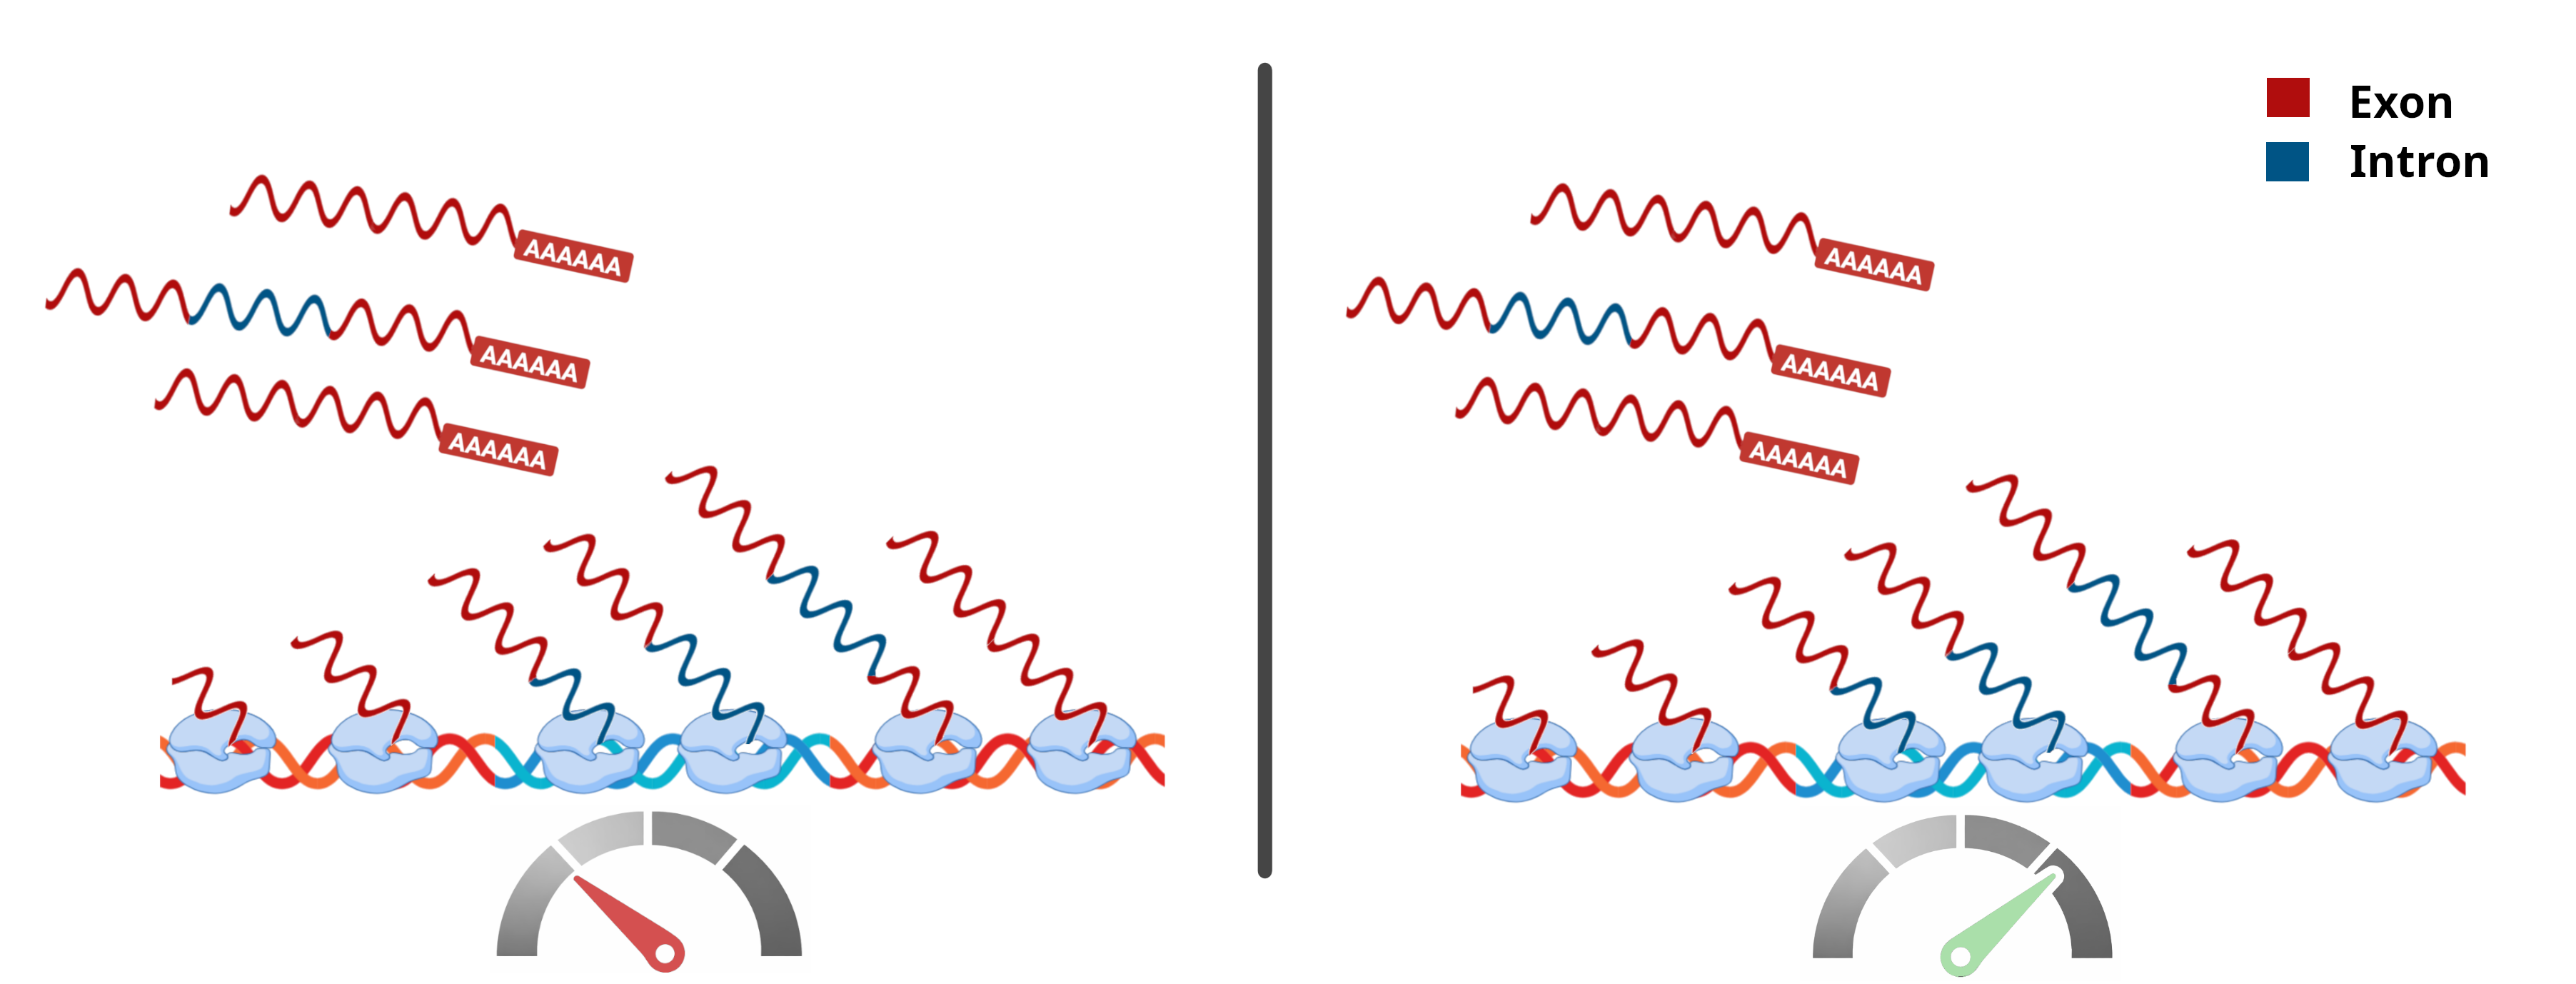
\includegraphics[width=11cm]{invariance}
		\end{center}	
		
	\end{frame}	
	
	\begin{frame}
		\frametitle{Estimating LFCs of kinetic rates}
		\pause
		\begin{itemize}
			\item The LFCs of kinetic rates are the parameters of my model.
			\pause
			\item I ignored the LFC of RNA degradation so far; as shown above, LFCs of all rates are not jointly identifiable anyway.
			\pause
			\item Observations are the read counts (exonic and intronic), and locations (i.e., histogram) of intronic reads.
			\pause
			\item Loss function = negative log-likelihood of the model (function of parameters, given the observations).
		\end{itemize}
	\end{frame}	
	
	\begin{frame}
		\frametitle{Loss minimization}
		\pause
		\begin{itemize}
			\item We want to minimize the loss function $L \colon \mathbb{R}^p \to \mathbb{R}$, where $\theta \in \mathbb{R}^p$ is a p-dimensional set of parameters.
			\begin{center}
				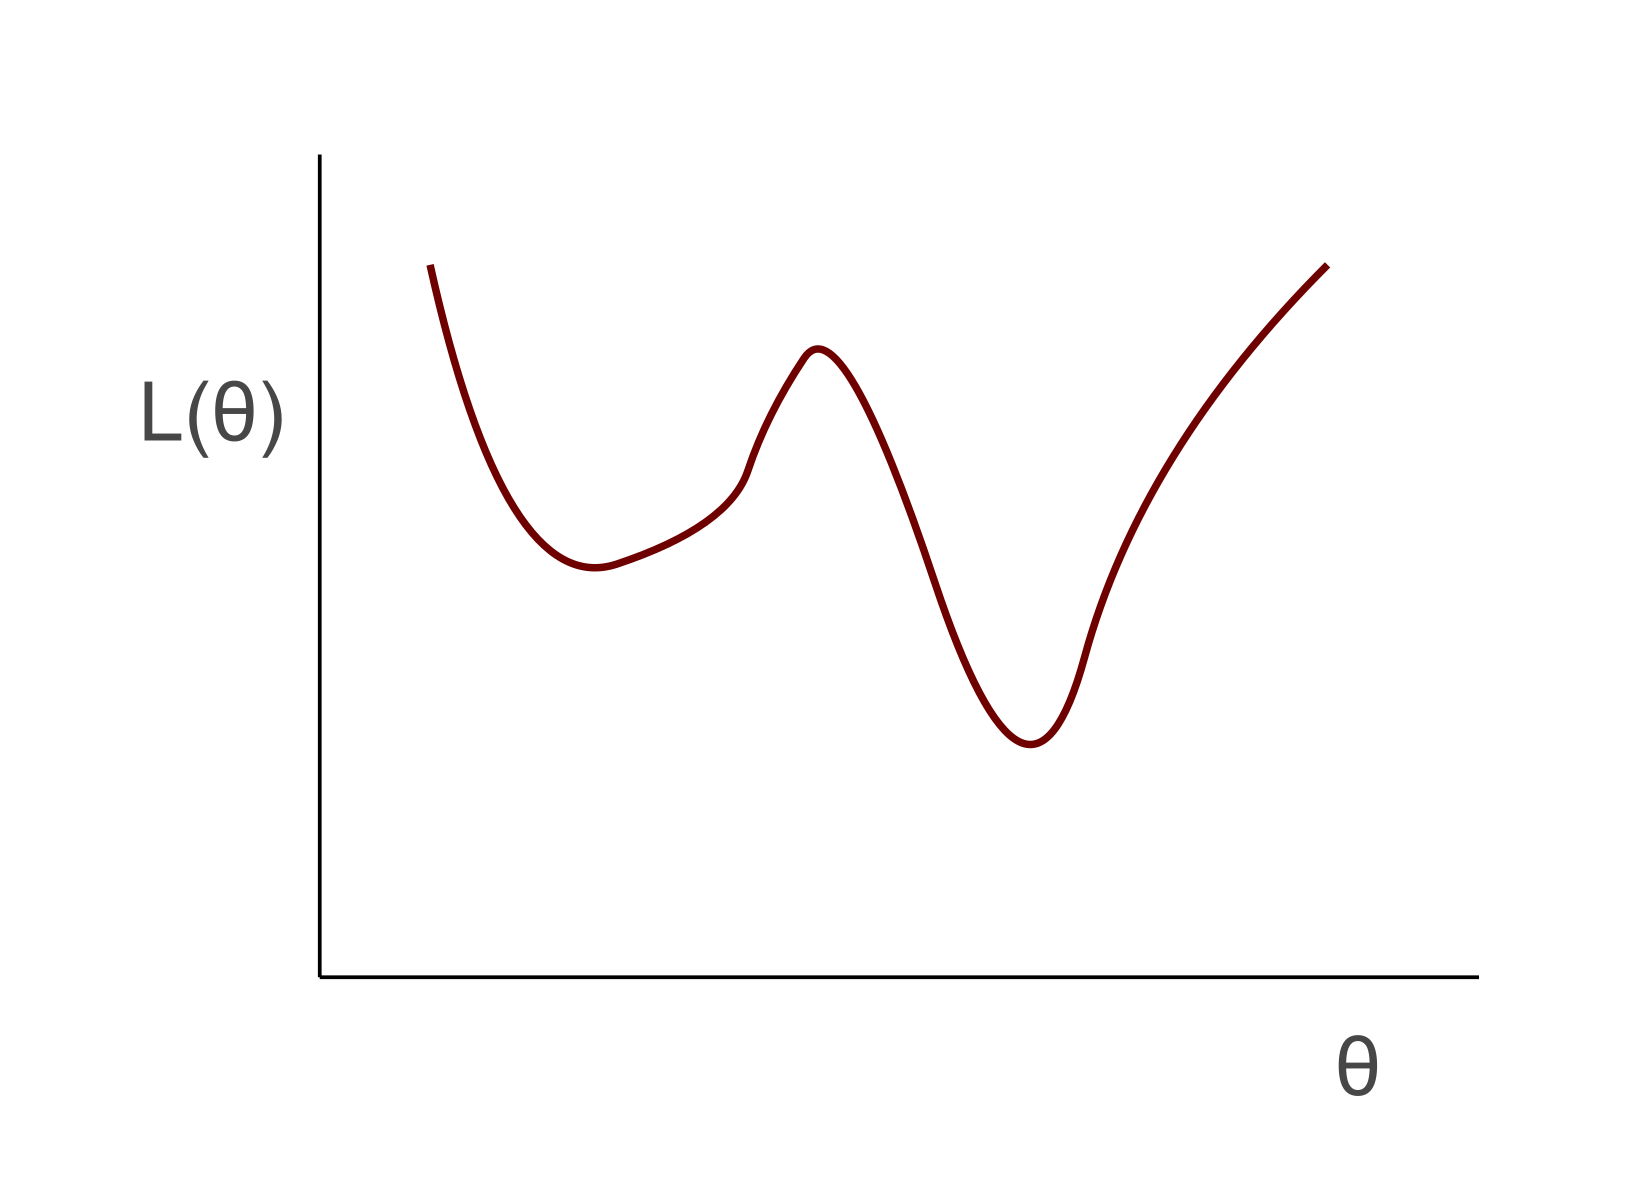
\includegraphics[width=6cm]{loss}
			\end{center}
			\pause
			\item The loss function is non-convex, and may have multiple local minima.
			\pause
			\item Gradient-based methods (e.g., L-BFGS algorithm) may get stuck in local minima. Is there a way to always find the global minimum of a non-convex function? 
			\pause
			\begin{itemize}
				\item Yes! (With some effort).
			\end{itemize}
		\end{itemize}
	\end{frame}	
	
	
	
	
	\begin{frame}
		\frametitle{The End}
		Thank you for your attention!
		
		\begin{center}
			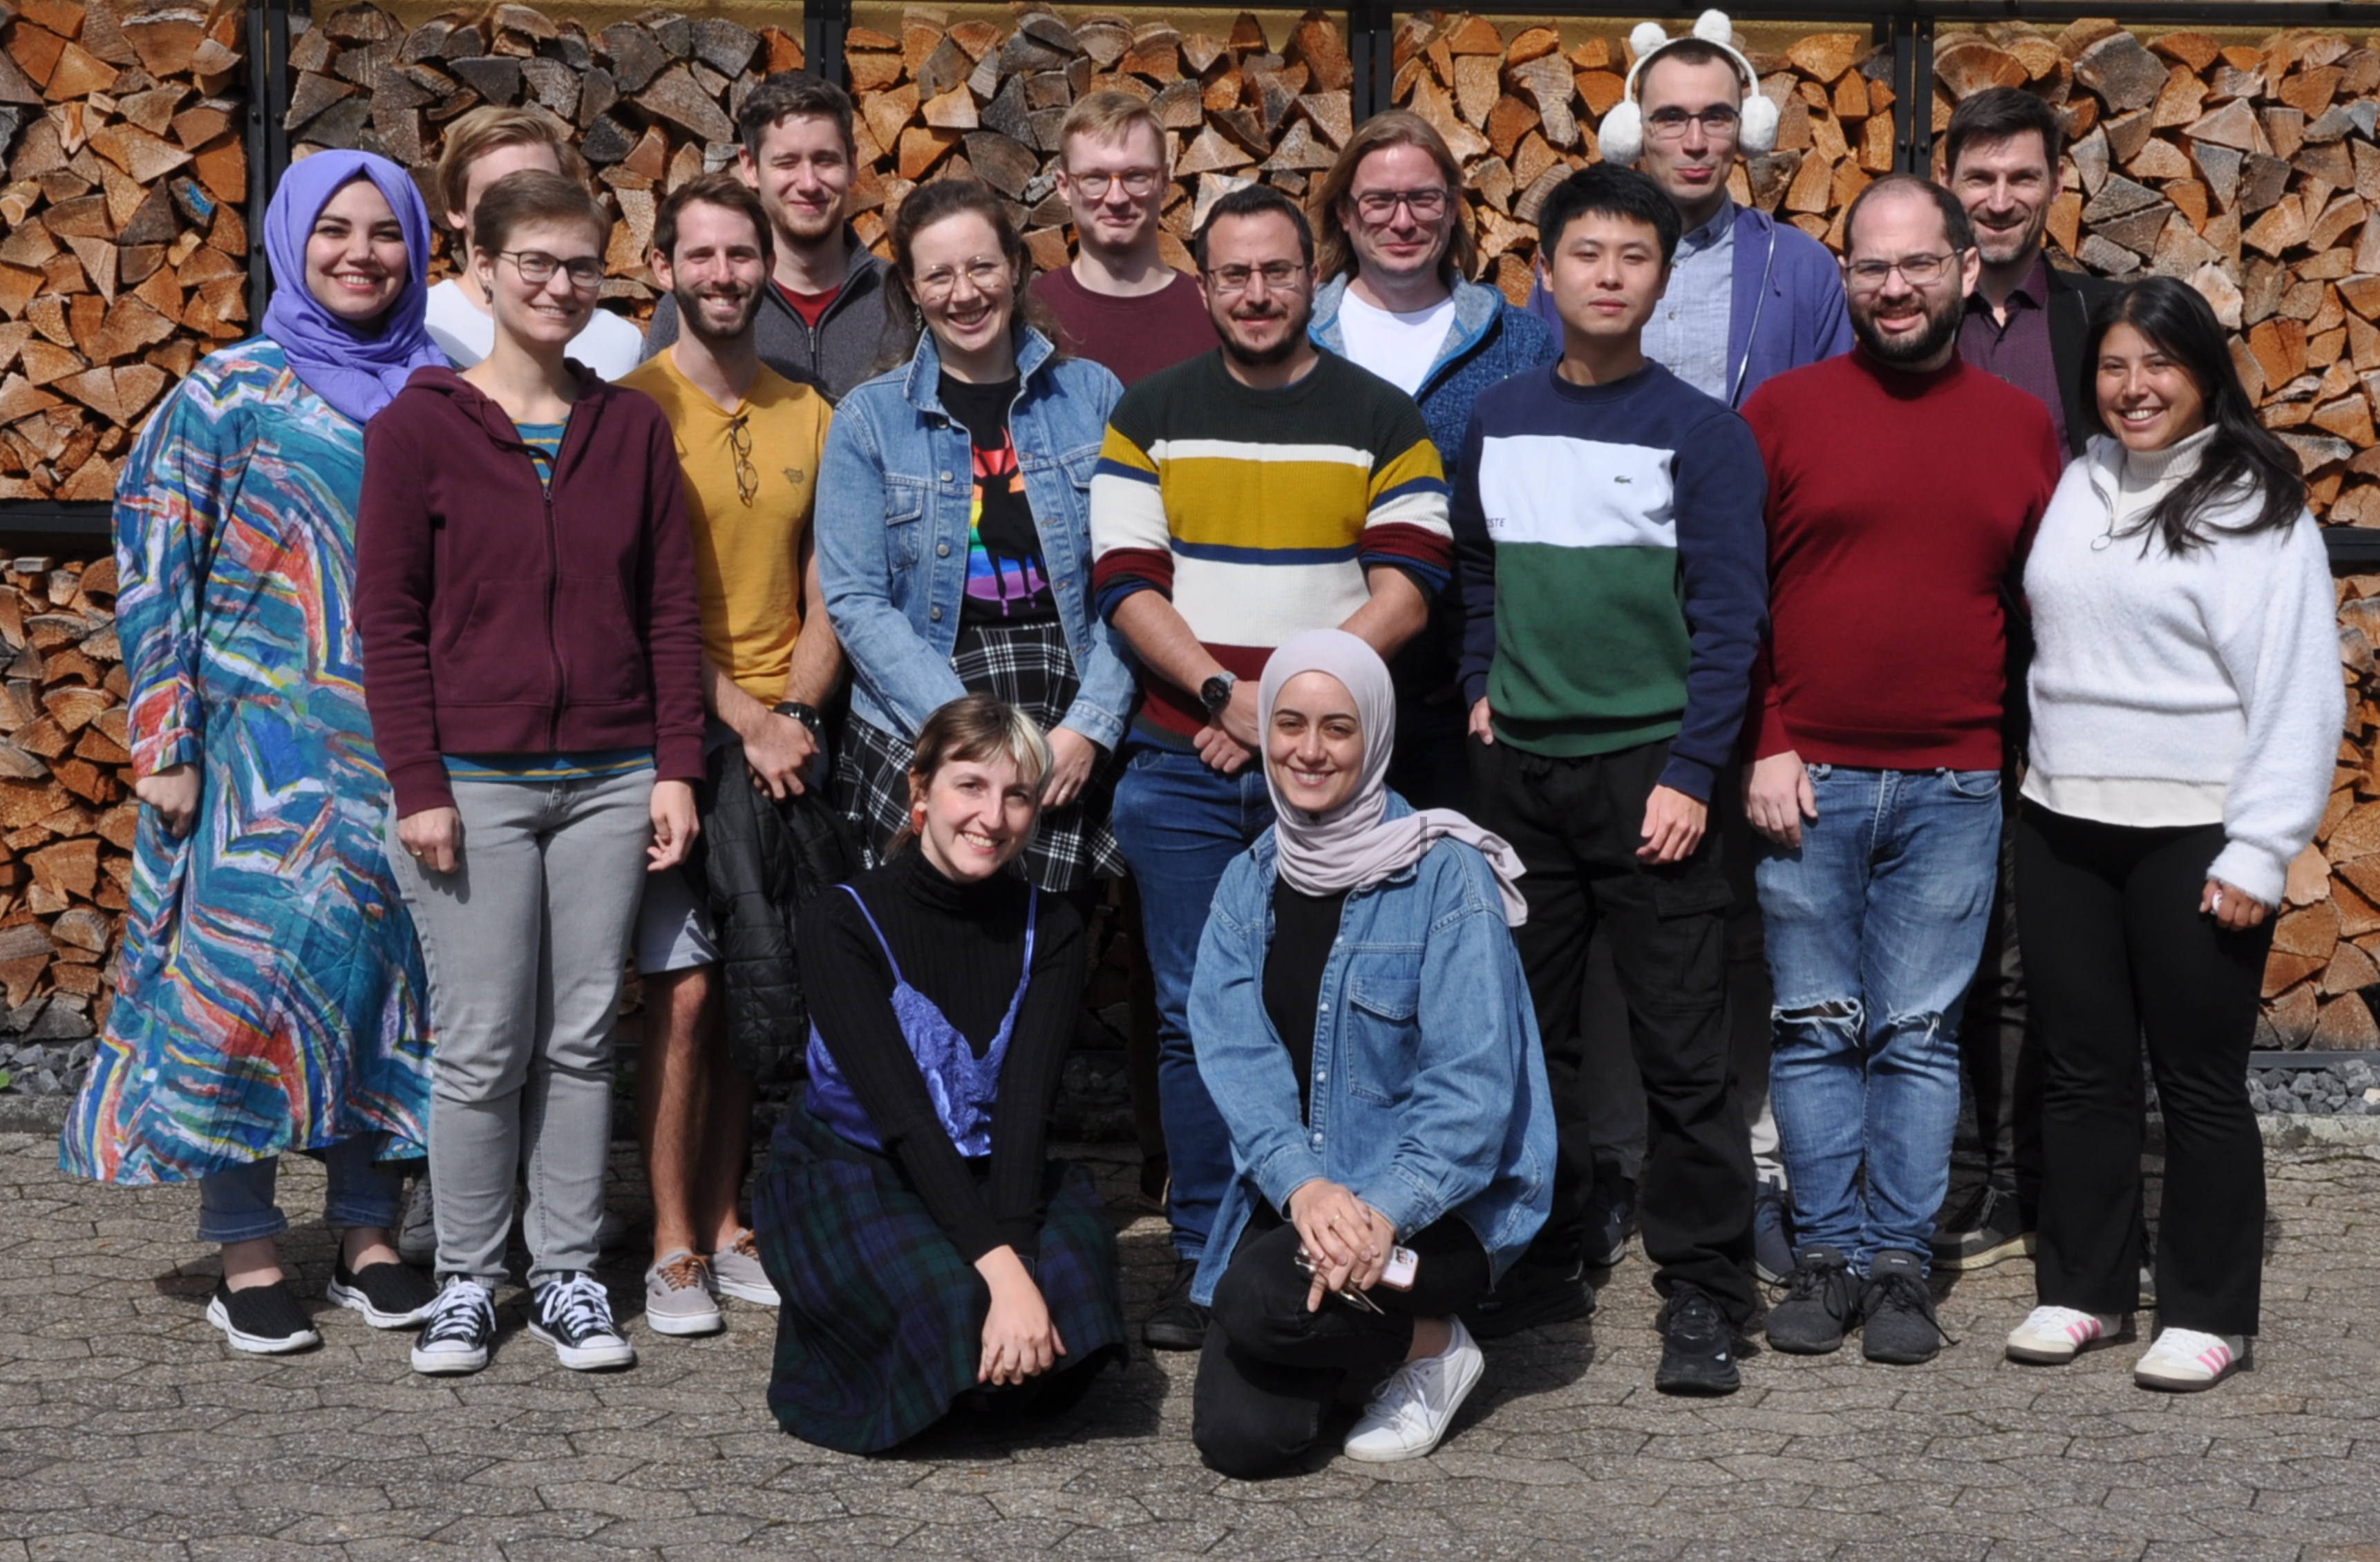
\includegraphics[width=9cm]{group_picture}		
		\end{center}
		
		\tiny{Illustrations in the presentation were created using BioRender.}
	\end{frame}
	
	
	
\end{document}
